\chapter{ENCOUNTERS}

\begin{multicols}{2}

\index{Encounters}An encounter is broadly defined as an interaction between player characters and GM controlled elements presenting the possibility to bring meaningful changes, for good or ill, to the PCs based on their decisions.  A simple, mundane action, like purchasing goods or setting up camp, isn't an encounter. However, if unknown variables are added (the merchant offers a cursed artifact, or assassins wait in the shadows), it becomes an encounter to be played out.   Player decision is always a major element in encounters.  Forcing PCs into an inescapable situation where they cannot act isn't an encounter (it is, however, poor game design), and interaction between player characters isn't considered an encounter either.  Encounters don't have to present an element of danger, although it's usually a factor, even if only in some indirect manner.  

\index{Encounters!Planned}\section{PLANNED ENCOUNTERS}

The GM prepares planned encounters before the session.  The two kinds of planned encounters are keys and triggers.

\paragraph{Key:} The key describes the encounter, what is found there, and how it may react to the PCs.  Keys include a description of creatures or NPCs that may be in the area, traps, treasure, and other special conditions that may or may not affect the players. Descriptions such as sights, smells, and sounds may be included.  

Keys are static; what the GM writes is what happens.  This can lead to illogical problems depending, for example, on the time of day or events that happen in other areas.  It's impossible to plan for every situation, so the best way to avoid these problems is to make general notes, not specific details.  

\paragraph{Trigger:} A trigger is a simple statement that serves as a reaction to an action.  It can be used as part of a key or by itself.  Triggers are broader than keys in that they cover actions the PCs might take.  When designing a trigger, think of the most important actions a character might do (investigating, searching, questioning people, etc.) and write up reactions to them.  Triggers are more difficult than keys because they cover an even broader range of possibilities.  GMs are expected to improvise for situations they may not have covered.

\subsection{COMBINING KEYS AND TRIGGERS}

The most dynamic (and challenging) method of writing planned encounters is combining keys and triggers.  The key includes the basic description of the area and its inhabitants, while the trigger describes how the key will react to the player's intervention.  While no planned encounter can cover every situation, this system provides the best setup but requires more work.  

An example planned encounter can be seen below.  The first paragraph serves as the key; static information such as the location, sights, and smells are listed.  The second paragraph serves as the trigger; it describes what can be found at what time and how the encounter reacts to the players.

\paragraph{Giant's Cave:} This circular room, 80' in circumference with a 30' tall ceiling, is carved into the side of a hill.  It's musty and damp with moss covered walls and poor ventilation.  At the far end is a makeshift bed made from dirty rags and animal skins.  Boog, the hill giant, calls this cave his home.  He always keeps a dirty sack full of makeshift utensils, 100 gp, and a golden idol (worth 500 gp) under his bed.

At night Boog is found passed out drunk in his bed ($-1$ to attack rolls and a penalty to wisdom checks).  During the day Boog hunts and sets a simple snare trap at the cave entrance (the trap ensnares and dangles from the ceiling anyone who steps on it).  Boog prefers to take prisoners, whom he eats at a later date.  He grabs his hidden stash and runs when reduced to half his hit points.  

\index{Encounters!Random}\section{RANDOM ENCOUNTERS}

Random encounters add variety to the game.  When appropriate, the GM makes a check to determine if the party encounters something.  Random encounters can include NPCs and monsters, friendly or hostile, and special situations like observing a battle in the distance or walking through a trapped field.  

The GM sets how often he checks a random encounter table and the chance of a random encounter happening (5\% every hour, 10\% every 24 hours, etc.).  Creatures encountered should be relative to the PCs power.  Random encounters don't have to include creatures at all; a gust of wind that blows out torches, clattering rocks, or howls in the distance help build tension and all make good additions to an encounter chart.  GMs should not feel restricted by random encounter charts; in some cases they can be illogical or detract from the fun of the game.  

Random encounter tables can be made from any combination of die rolls but the most common are the 2--20 and percentile table.  Monster or events are added to the table based on their frequency appearing.  

\noindent
\begin{minipage}{\columnwidth}

\captionof{table}{Encounter Frequency}\label{encounterfreq}
\noindent
\begin{tabular}{|p{.6\columnwidth}|p{.3\columnwidth}|}
\hline
Frequency	& 1d100 \\
\hline\hline
\rowcolor[gray]{.9}Common		& 01--70 \\
Uncommon	& 71--90 \\
\rowcolor[gray]{.9}Rare		& 91--97 \\
Very rare	& 98--00 \\
\hline
\end{tabular}

\end{minipage}

\subsection{2--20 TABLE}

The 2--20 table presents a possible 19 different encounters.  Begin by categorizing monsters by \index{Encounters!Frequency}frequency (listed under their stat blocks) and assign them to the table.  When checking the chart, roll 1d12~+~1d8 to generate a number between 2 and 20. 

\noindent
\begin{minipage}{\columnwidth}

\captionof{table}{2--20 Table}\label{twototwentytable}
\noindent
\begin{tabular}{|p{.3\columnwidth}|p{.6\columnwidth}|}
\hline
1d12~+~1d8	& Creature Frequency \\
\hline\hline
\rowcolor[gray]{.9}2	& Very rare \\
3	& Very rare \\
\rowcolor[gray]{.9}4	& Very rare/rare \\
5	& Rare \\
\rowcolor[gray]{.9}6	& Rare \\
7	& Uncommon* \\
\rowcolor[gray]{.9}8	& Uncommon* \\
9	& Common** \\
\rowcolor[gray]{.9}10	& Common** \\
11	& Common** \\
\rowcolor[gray]{.9}12	& Common** \\
13	& Common** \\
\rowcolor[gray]{.9}14	& Uncommon* \\
15	& Uncommon* \\
\rowcolor[gray]{.9}16	& Rare \\
17	& Rare \\
\rowcolor[gray]{.9}18	& Very rare/rare \\
19	& Very rare \\
\rowcolor[gray]{.9}20	& Very rare \\
\hline
\end{tabular}
\noindent\begin{tabular}{p{.95\columnwidth}}
*Or two very rare creatures, 50\% chance for either \\
**Or two rare creatures, 50\% chance for either \\
\end{tabular}\vspace{.5em}

\end{minipage}

\subsection{PERCENTILE TABLE}

A percentile table is created when the GM divides the number of monsters in a frequency category by their frequency percentage to come up with a variable range.  For example, in a percentile table with seven common monsters, each monster would have a 10\% chance of being encountered.  The higher the percentile rolled, the rarer the creature encountered.  Percentile tables take longer to set up but allow more customization of encounters.

\noindent
\begin{minipage}{\columnwidth}

\captionof{table}{Example Percentile Table}\label{examplepercentile}
\noindent
\begin{tabular}{|p{.3\columnwidth}|p{.6\columnwidth}|}
\hline
1d100		& Creature \\
\hline\hline
\rowcolor[gray]{.9}Common		& \\
\rowcolor[gray]{.9}\hspace{2em}1--8	& Creature 1 \\
\hspace{2em}9--16	& Creature 2 \\
\rowcolor[gray]{.9}\hspace{2em}17--24	& Creature 3 \\
\hspace{2em}25--32	& Creature 4 \\
\rowcolor[gray]{.9}\hspace{2em}33--40	& Creature 5 \\
\hspace{2em}41--48	& Creature 6 \\
\rowcolor[gray]{.9}\hspace{2em}49--56	& Creature 7 \\
\hspace{2em}57--64	& Creature 8 \\
\rowcolor[gray]{.9}\hspace{2em}65--72	& Creature 9 \\
Uncommon	& \\
\hspace{2em}73--78	& Creature 10 \\
\rowcolor[gray]{.9}\hspace{2em}79--84	& Creature 11 \\
\hspace{2em}85--91	& Creature 12 \\
\rowcolor[gray]{.9}Rare		& \\
\rowcolor[gray]{.9}\hspace{2em}92--95	& Creature 13 \\
\hspace{2em}96--99	& Creature 14 \\
\rowcolor[gray]{.9}Very Rare	& \\
\rowcolor[gray]{.9}\hspace{2em}00		& Creature 15 \\
\hline
\end{tabular}

\end{minipage}

\section{DUNGEON ENCOUNTERS}

Dungeons are given a designated level, which represents the relative power of creatures encountered.  Although any creature can populate a dungeon, creatures encountered shouldn't be more than two levels above or below the dungeon level.  Creatures encountered in a dungeon are grouped into levels based on their experience value.  For each level above or below the dungeon level, the creature's frequency rating shifts up---weak creatures will avoid high-level dungeons where strong creatures tend to gather. Therefore, if an uncommon, rare or very rare encounter is rolled, the GM could use a higher-level, equal-level, or lower-level encounter.

Although a dungeon's level should correspond with the PC's level, there's never any guarantee that a dungeon will be safe or easily conquered.

\noindent
\begin{minipage}{\columnwidth}

\captionof{table}{Creature Level}\label{creaturelevel}
\noindent
\begin{tabular}{|p{.45\columnwidth}|p{.45\columnwidth}|}
\hline
XP	& Creature Level \\
\hline\hline
\rowcolor[gray]{.9}1--20	& 1 \\
21--50	& 2 \\
\rowcolor[gray]{.9}51--150	& 3 \\
151--250	& 4 \\
\rowcolor[gray]{.9}251--500	& 5 \\
501--1,000	& 6 \\
\rowcolor[gray]{.9}1,001--3,000	& 7 \\
3,001--5,500	& 8 \\
\rowcolor[gray]{.9}5,501--10,000	& 9 \\
10,001+	& 10 \\
\hline
\end{tabular}

\end{minipage}

\noindent
\begin{minipage}{\columnwidth}

\captionof{table}{Sample Dungeon Level 3}\label{sampledungeon3}
\noindent
\begin{tabular}{|p{.25\columnwidth}|p{.35\columnwidth}|p{.25\columnwidth}|}
\hline
1d12~+~1d8	& Creature Frequency	& Creature Level \\
\hline\hline
\rowcolor[gray]{.9}2	& Very rare	& 6 \\
3	& Very rare	& 4 \\
\rowcolor[gray]{.9}4	& Very rare/rare	& 3 \\
5	& Rare	& 1 \\
\rowcolor[gray]{.9}6	& Rare	& 4 \\
7	& Uncommon	& 2 \\
\rowcolor[gray]{.9}8	& Uncommon	& 3 \\
9	& Common	& 3 \\
\rowcolor[gray]{.9}10	& Common	& 3 \\
11	& Common	& 3 \\
\rowcolor[gray]{.9}12	& Common	& 3 \\
13	& Common	& 3 \\
\rowcolor[gray]{.9}14	& Uncommon	& 4 \\
15	& Uncommon	& 2 \\
\rowcolor[gray]{.9}16	& Rare	& 5 \\
17	& Rare	& 1 \\
\rowcolor[gray]{.9}18	& Very rare/rare	& 6 \\
19	& Very rare	& 1 \\
\rowcolor[gray]{.9}20	& Very rare	& 6 \\
\hline
\end{tabular}

\end{minipage}

\subsection{DUNGEON TRAPS AND TRICKS}

Perhaps the most unique encounters in dungeons are tricks and traps.  These are obstacles that are hidden or require interaction to overcome.  They can be harmless but impeding or deadly.  XP, based on the difficulty, should be awarded for disabling or overcoming traps and tricks but only if the party is aware and deliberate of their actions.  Triggering a crossbow obviously ruins the trap but if the PCs discover the hidden crossbow and cut the trip wire, they should be awarded XP for it.

GMs are encouraged to be flexible and creative when creating them.  A trap or trick should have a logical way to overcome them.  Instant-death and unavoidable traps are frustrating and cumbersome to deal with.  Likewise, logic puzzles and riddles are usually so obscure that they should be used with caution if they're the only means of players progressing.  For example:

\begin{itemize}

\item Giant bubbles rove about.  Contact with them envelopes large-sized or smaller characters, inflicting 1d6 points of damage each round as they suffocate.  A bubble can be popped with at least 1 point of damage by a piercing weapon but there's a 50\% chance the person inside is damaged as well.  There's a 25\% chance a bubble has a gem inside.

\item Statues animate when approached.  Possible actions are pointing towards treasure (or danger), reciting a poem, scream, or swing at anyone too close.

\item One-way doors, sliding fireplaces, a set of stairs that become a flat slope, bookshelves that open when a book is pulled, etc.

\item Rooms that are actually elevators connecting multiple floors.  The rooms will shift floors when people enter, potentially throwing off mappers.

\item Four-way passageways which slide imperceptibly around, causing wanderers to get turned around.

\item Intelligent monsters that grow patches of screeching mushrooms.

\end{itemize}

\noindent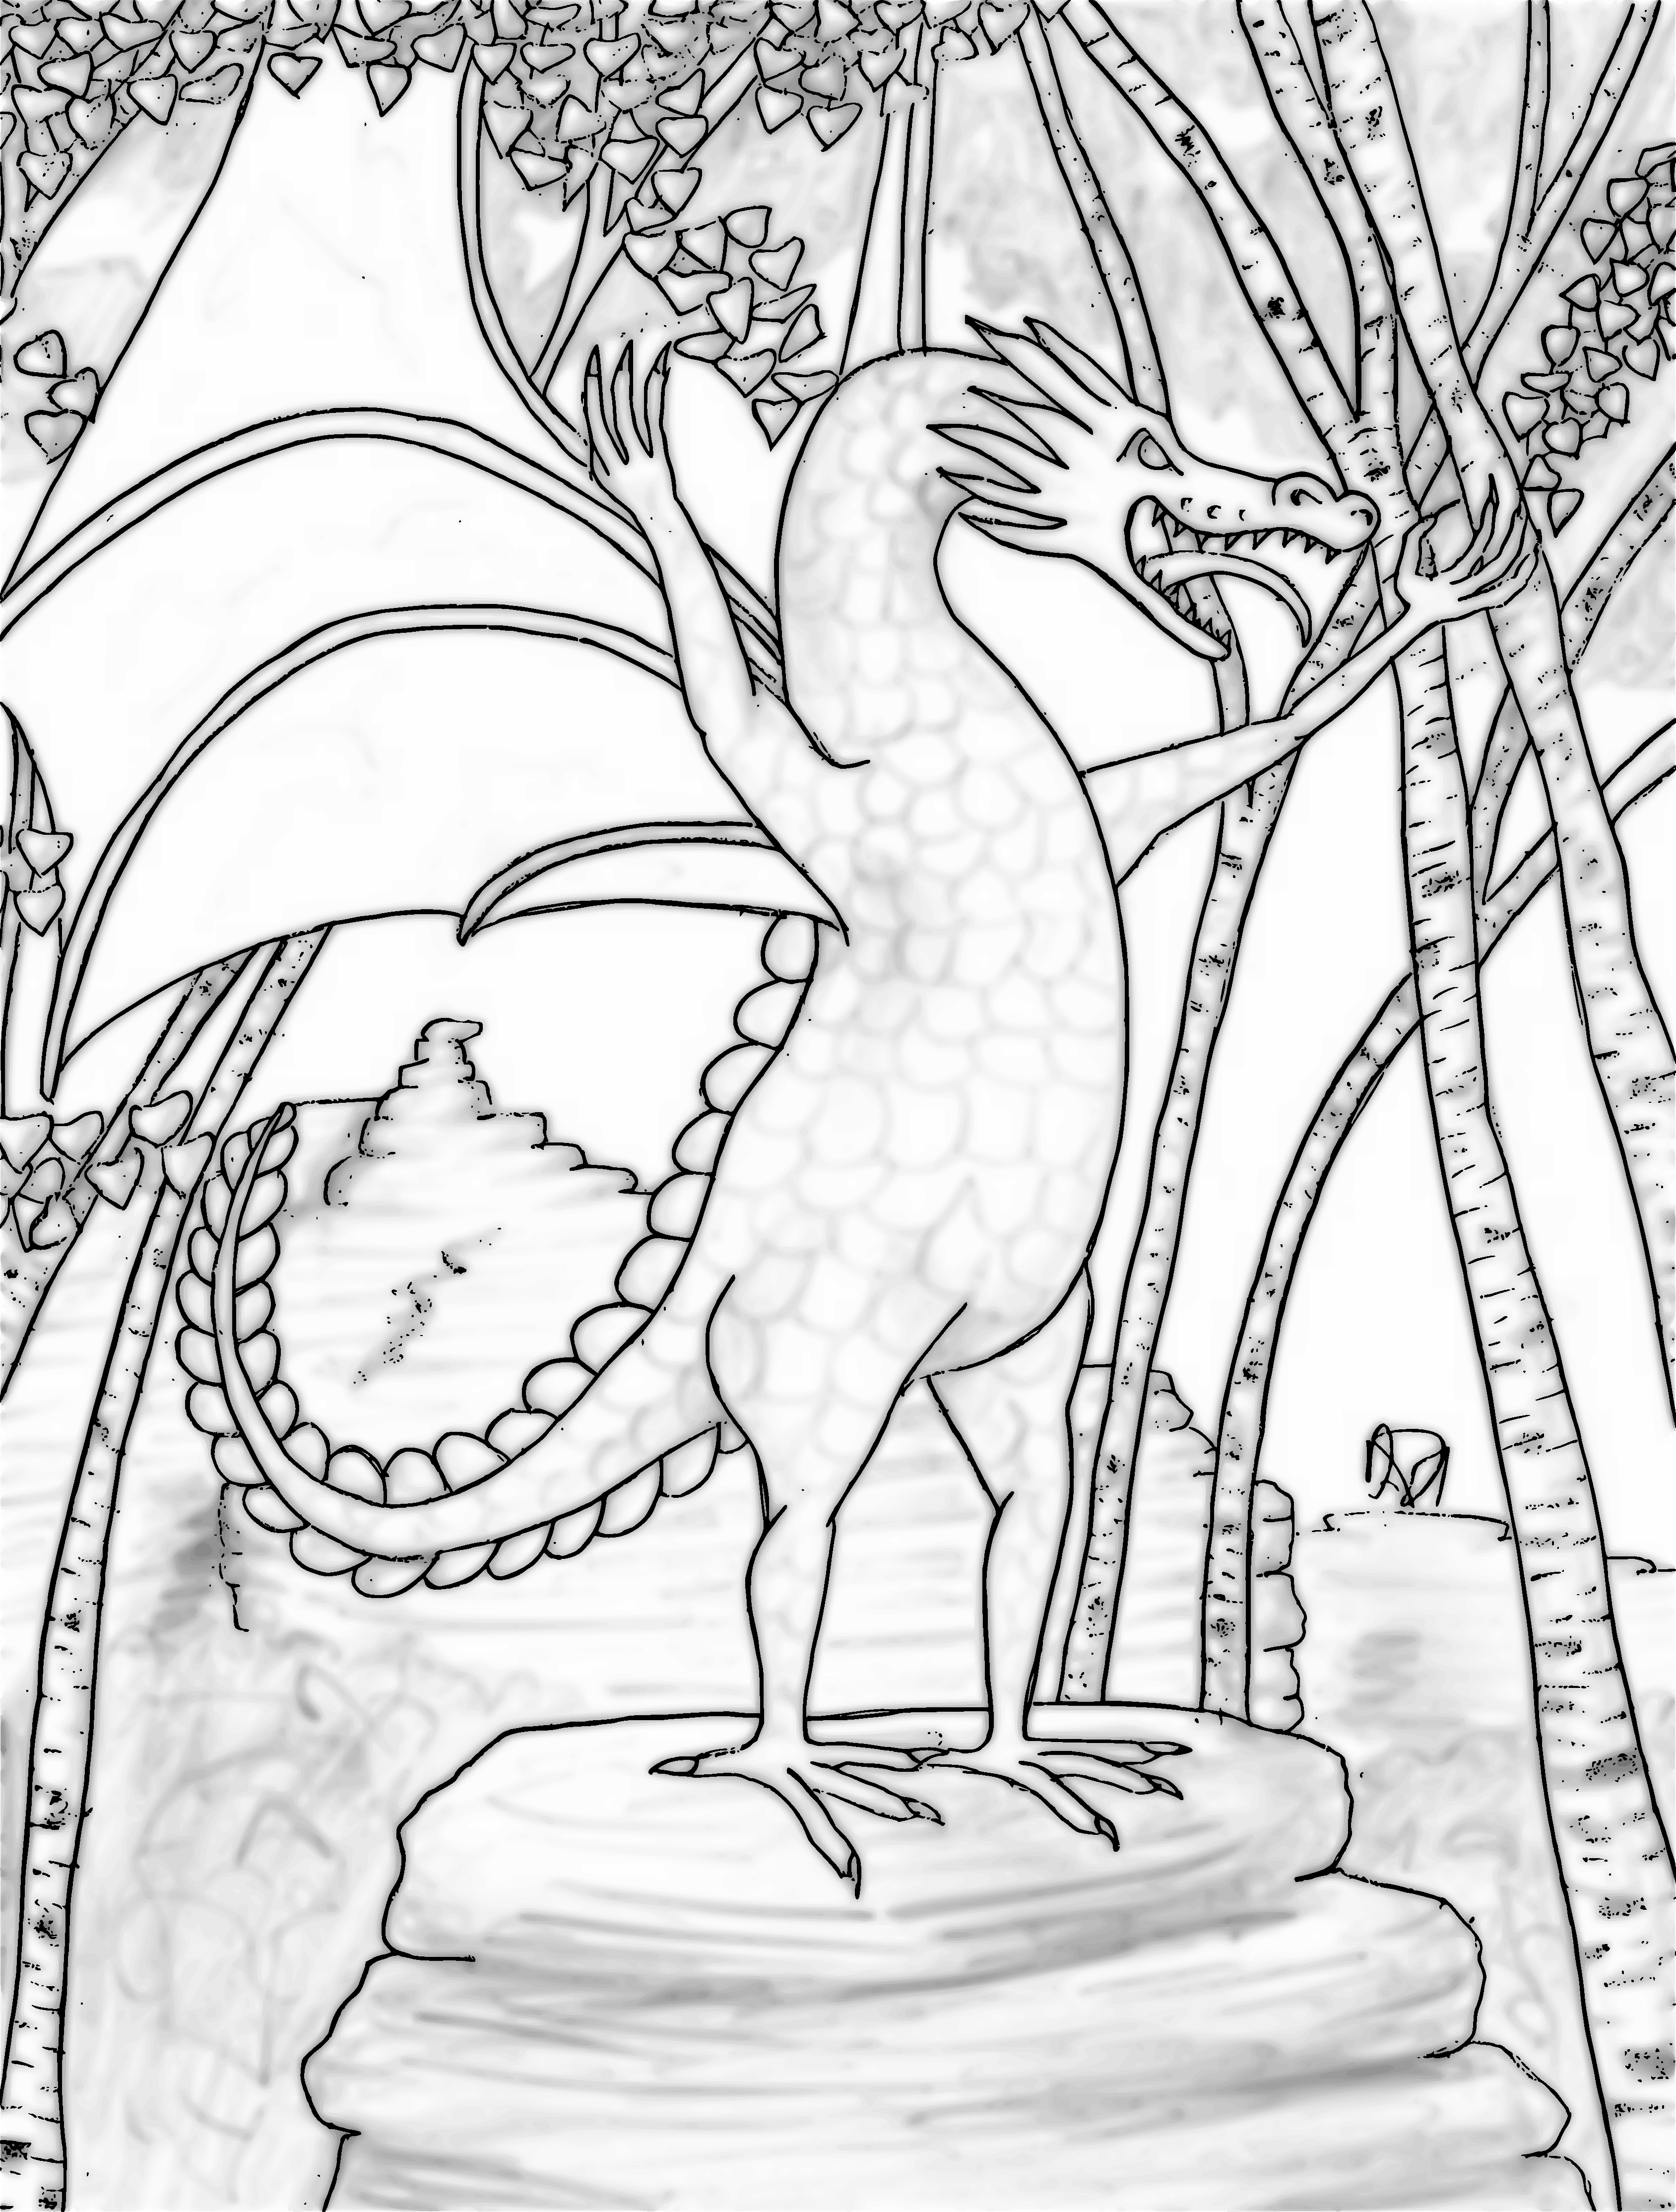
\includegraphics[width=\columnwidth]{marshfield.pdf}\label{marshfield} 

\section{WILDERNESS ENCOUNTERS}

Wilderness encounters are more dangerous than dungeon encounters because there is no rating of power for monsters to conform to.  Hilly lowlands can contain anything ranging from goblins to trolls and dragons.  Special consideration should be made to ensure PCs don't encounter higher-level creatures without some means of escape.  If a low-level party would normally encounter a band of hill giants, they should instead stumble upon them counting the bounty of a recent raid while safely hiding in the bushes.  If the PCs wish to risk their lives they can make that choice, but forcing them into an untenable fight is poor refereeing.  

Wilderness encounters should be categorized by region and other environmental factors.  The farmlands of a civilized area will contain more encounters with patrolling guards and merchants than wild monsters, although bandits and other opportunistic creatures might slip by.  A dry, sandy desert will have different encounters than a semi-arid desert.  The creatures encountered in a freshwater lake likely wouldn't be encountered in a saltwater sea.

\section{SPECIAL ENCOUNTER TABLES}

Encounter tables don't have to be limited to wilderness and dungeon.  Towns and other areas of civilization can include their own encounters.  These encounters could involve various events (runaway donkey cart), encounters with diseased beggars asking for alms, friendly merchants peddling mysterious goods, questioning guards, or frustrated nobility.  While towns and smaller civilizations can use the same table, most cities have distinctive districts and jurisdictions, each needing its own encounter table. 

\section{ENCOUNTER CHECKS}

\index{Encounters!Encounter Checks}The GM is tasked with determining when a random encounter might take place.  The terrain type determines when an encounter check is made.   The time of day and other environmental factors can also modify this roll.  The following table is a generalized chart designed to give GMs a basic idea of when they should make an encounter check based on the time of day (24 hour clock) and terrain.

\paragraph{Encounter Check:} If the result of a 1d10 is equal to or less than the listed number, the GM rolls on a random encounter chart.

\paragraph{Time of Day:} If an ``X" is listed under the specified time, the GM rolls an encounter check.  

\paragraph{Populated Area Checks:} The chart assumes an unpopulated wilderness.  If the area is sparsely patrolled or populated by civilized creatures, the chance of an encounter increases by 1.  If the area is densely populated or regularly patrolled, the chance of an encounter increases by 2.  Likewise, the PCs are much more likely to encounter civilized creatures than monsters in these areas.

\paragraph{Dungeon Checks:} Dungeon checks don't follow the chart and occur more frequently.  Every hour, the GM rolls 1d10, and a random dungeon encounter occurs on a result of 1.  This chance can increase in particularly dangerous areas.  If the PCs make excessive noise or otherwise draw attention, a check should be made immediately.

\subsection{ENCOUNTER SIZE}

When an encounter is determined, the GM determines the number of creatures encountered.  Monsters list a typical encounter size, but this guideline doesn't have to be followed explicitly.  As a general rule, it's better to have a small encounter than a large one that can easily overwhelm the PCs.  Large predators often hunt alone or in small packs, while smaller predators prefer larger packs.  Herbivores and other normally docile animals form into herds and may stampede wildly when disturbed.  Intelligent creatures can be encountered in any number, ranging from solitary scouts to hunting parties and war bands.

\end{multicols}

\noindent
\begin{minipage}{\columnwidth}

\captionof{table}{Terrain Encounter Checks}\label{terrainencounter}
\noindent
\begin{tabular}{|p{.1\textwidth}|p{.1\textwidth}|p{.1\textwidth}|p{.1\textwidth}|p{.1\textwidth}|p{.1\textwidth}|p{.1\textwidth}|p{.1\textwidth}|}
\hline
Terrain	& Check	& 0300--0600 	& 0700--1000	& 1100--1400	& 1500--1800	& 1900--2200	& 2300--0200 \\
\hline\hline
\rowcolor[gray]{.9}Plains		& 1	& X		& --	& X		& --	& X		& -- \\
Scrub/brush	& 1	& X		& --	& X		& X		& --	& X \\
\rowcolor[gray]{.9}Forest		& 2	& X		& X		& X		& X		& X		& X \\
Desert		& 1	& X		& --	& --	& X		& --	& X \\
\rowcolor[gray]{.9}Hills		& 2	& --	& X		& --	& X		& --	& X \\
Mountains	& 3	& X		& --	& --	& X		& X		& -- \\
\rowcolor[gray]{.9}Swamp		& 4	& X		& X		& X		& X		& X		& X \\
Jungle		& 3	& X		& X		& X		& X		& X		& -- \\
\rowcolor[gray]{.9}Ocean		& 1	& --	& X		& --	& --	& X		& -- \\
Arctic		& 1	& --	& --	& X		& X		& --	& -- \\
\hline
\end{tabular}

\end{minipage}

\noindent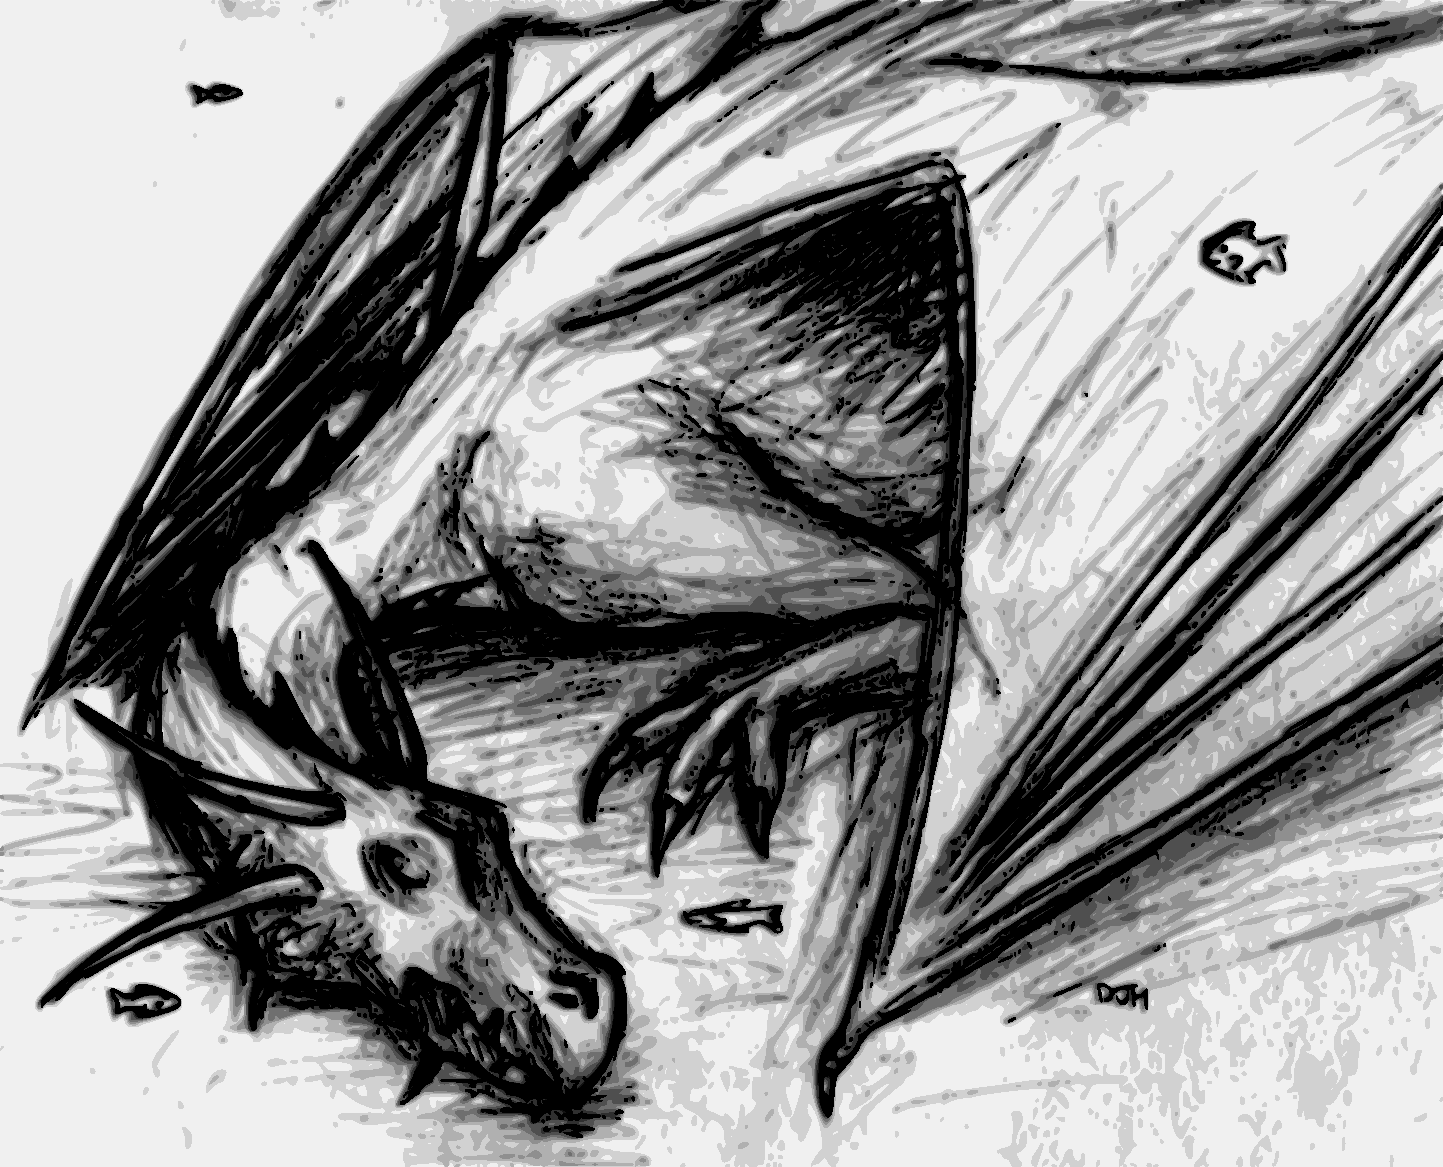
\includegraphics[width=.99\textwidth]{sarkothion.pdf}\label{sarkothian}

\begin{multicols}{2}

\section{SURPRISE}

\index{Surprise}When one party has a chance of being caught off guard, they roll a surprise check.  A surprise check is a roll of 1d10; on a 1, 2, or 3 the party is surprised.  Surprise is based on party awareness.  If a party is aware of their opponents they likely won't be surprised.  The GM decides when a party can be surprised or if individual characters roll surprise rolls.  The following table shows possible modifiers to the surprise roll of a specific party.

It's possible to set up an ambush.  If the opponents are unaware, the ambushing party gets a free round to attack.  The ambushed party must also roll a surprise check to determine if they are surprised allowing the ambushing party to possibly get two free rounds of actions.
 
\subsection{THE SURPRISE ROUND}

While a character is surprised, all unsurprised characters receive free actions.  These actions can include anything they're capable of in a normal combat round with the exception of spell casting.  For example, using a wand of fireballs is allowed, but a wizard cannot cast a fireball spell.  \index{Armor Class!Effects of Surprise}Surprised characters lose their dexterity bonus to AC during the surprise round.  Initiative is rolled if opposing individuals are not surprised.

Unsurprised parties can use the surprise round to escape if they choose, but their success depends on their opponent's movement value.  If neither or both parties are surprised, combat begins normally by rolling initiative.

\noindent
\begin{minipage}{\columnwidth}

\captionof{table}{Surprise Modifiers}\label{surprisemodifiers}
\noindent
\begin{tabular}{|p{.6\columnwidth}|p{.3\columnwidth}|}
\hline
Conditions	& Modifier \\
\hline\hline
\rowcolor[gray]{.9}The opponent party is	& \\
\hspace{2em}Magically silenced	& $-2$ \\
\rowcolor[gray]{.9}\hspace{2em}Invisible	& $-2$ \\
\hspace{2em}Distinct odor	& +2 \\
\rowcolor[gray]{.9}\hspace{2em}Per 10 members	& +1 \\
\hspace{2em}Camouflaged	& $-1$ to $-3$ \\
\rowcolor[gray]{.9}The party/individual is	& \\
\rowcolor[gray]{.9}\hspace{2em}Fleeing	& $-2$ \\
\hspace{2em}In poor lighting	& $-1$ \\
\rowcolor[gray]{.9}\hspace{2em}In darkness	& $-4$ \\
\hspace{2em}Panicked	& $-2$ \\
\rowcolor[gray]{.9}\hspace{2em}Anticipating attack*	& +2 \\
\hspace{2em}Suspicious*	& +2 \\
\rowcolor[gray]{.9}Special Conditions	& \\
\rowcolor[gray]{.9}\hspace{2em}Rain	& $-1$ \\
\hspace{2em}Heavy fog	& $-2$ \\
\rowcolor[gray]{.9}\hspace{2em}Extremely still**	& +2 \\
\hline
\end{tabular}
\noindent\begin{tabular}{p{.95\columnwidth}}
*Anticipating attack means the party has good reason to believe an attack will happen in a specific area or direction. It's not enough to simply anticipate an attack at all times. A suspicious party has reason to believe another group might try to make a hostile move. \\
** Assumes there's no noise or other slight distractions such as ambient sound and wind. \\
\end{tabular}\vspace{.5em}

\end{minipage}

\section{ENCOUNTER DISTANCE}

Although the distance at which creatures can be spotted and identified is quite far, it is rarely the case that any party will notice each other at these distances except on coverless terrain with ideal conditions.  The distance two groups may likely encounter each other normally is based on whether they're surprised and the terrain type.  In cases where there is no cover, the limit of sight is used.

\noindent
\begin{minipage}{\columnwidth}

\captionof{table}{Encounter Distance}\label{encounterdistance}
\noindent
\begin{tabular}{|p{.55\columnwidth}|p{.35\columnwidth}|}
\hline
Situation/Terrain	& Range in feet \\
\hline\hline
\rowcolor[gray]{.9}Both groups surprised	& 3d6 \\
One group surprised& 	4d6 \\
\rowcolor[gray]{.9}No surprise	 & \\
\rowcolor[gray]{.9}\hspace{2em}Smoke/heavy fog	& 6d6 \\
\hspace{2em}Jungle/dense forest	& 1d10~$\times$~10 \\
\rowcolor[gray]{.9}\hspace{2em}Light forest	& 2d6~$\times$~10 \\
\hspace{2em}Scrub, brush/bush	& 2d12~$\times$~10 \\
\rowcolor[gray]{.9}\hspace{2em}Grassland/little cover	& 5d10~$\times$~10 \\
\hspace{2em}Night or dungeon	& Limit of sight \\
\hline
\end{tabular}

\end{minipage}

\subsection{ENCOUNTER REACTION}

\index{Encounters!Reactions}Normally, creatures encountered have one of two reactions; hostile or passive.  Hostile creatures are looking to attack the other party regardless of the situation.  Passive creatures, while not necessarily friendly, are not looking to attack the other party (at least not at that exact moment).  A band of cutthroat bandits demanding the PC's gold in exchange for their lives is a passive party, as is a traveling merchant.

In situations where the GM doesn't have a group's reaction planned, he can roll on the reaction chart.  Roll 2d10, add any modifiers, and cross reference the following table based on the player character's disposition in relation to the opposing party.  Apply modifiers in accordance to the morale table.

\paragraph{Flight:} Seeks to avoid the characters or surrenders to them.

\paragraph{Friendly:} Seeks to help the characters (within reason) or holds no ill will.

\paragraph{Indifferent:} Is unconcerned with the characters and ignores them unless approached.  Will engage in small talk if pressed.

\paragraph{Cautious:} Is untrusting and suspicious of the characters, following or watching them closely.

\paragraph{Threatening:} Seeks to provoke or humiliate the characters but not necessarily cause harm.

\paragraph{Hostile:} Seeks to actively harm the characters whether through combat, intimidation, or humiliation.

Like morale, the reaction chart is an exception not a rule.  The GM is encouraged to use it only when he does not have an encounter planned.  The table shouldn't be relied on for every situation as the randomness can lead to illogical reactions.

\end{multicols}

\noindent
\begin{minipage}{\columnwidth}

\captionof{table}{Encounter Reactions}\label{encounterreact}
\noindent
\begin{tabular}{|p{.104\textwidth}|p{.194\textwidth}|p{.194\textwidth}|p{.194\textwidth}|p{.194\textwidth}|}
\hline
2d10		& Friendly	& Indifferent	& Threatening	& Hostile \\
\hline\hline
\rowcolor[gray]{.9}2 or less	& Friendly	& Friendly	& Friendly	& Flight \\
3			& Friendly	& Friendly	& Friendly	& Flight \\
\rowcolor[gray]{.9}4			& Friendly	& Friendly	& Cautious	& Flight \\
5			& Friendly	& Friendly	& Cautious	& Flight \\
\rowcolor[gray]{.9}6			& Friendly	& Friendly	& Cautious	& Cautious \\
7			& Friendly	& Indifferent	& Cautious	& Cautious \\
\rowcolor[gray]{.9}8			& Indifferent	& Indifferent	& Cautious	& Cautious \\
9			& Indifferent	& Indifferent	& Cautious	& Threatening \\
\rowcolor[gray]{.9}10			& Indifferent	& Indifferent	& Threatening	& Threatening \\
11			& Indifferent	& Indifferent	& Threatening	& Threatening \\
\rowcolor[gray]{.9}12			& Cautious	& Cautious	& Threatening	& Threatening \\
13			& Cautious	& Cautious	& Threatening	& Hostile \\
\rowcolor[gray]{.9}14			& Cautious	& Cautious	& Threatening	& Hostile \\
15			& Cautious	& Threatening	& Threatening	& Hostile \\
\rowcolor[gray]{.9}16			& Threatening	& Threatening	& Hostile		& Hostile \\
17			& Threatening	& Threatening	& Hostile		& Hostile \\
\rowcolor[gray]{.9}18			& Threatening	& Threatening	& Hostile		& Hostile \\
19			& Hostile		& Hostile		& Hostile		& Hostile \\
\rowcolor[gray]{.9}20			& Hostile		& Hostile		& Hostile		& Hostile \\
\hline
\end{tabular}

\end{minipage}

\noindent
\includegraphics[width=6.75in, height=2.5in]{testblock.pdf} 
